\documentclass{standalone}
\usepackage{tikz}
\usetikzlibrary{patterns, positioning}
\usepackage[sfdefault]{ClearSans} %% option 'sfdefault' activates Clear Sans as the default text font
\usepackage[T1]{fontenc}

\begin{document}
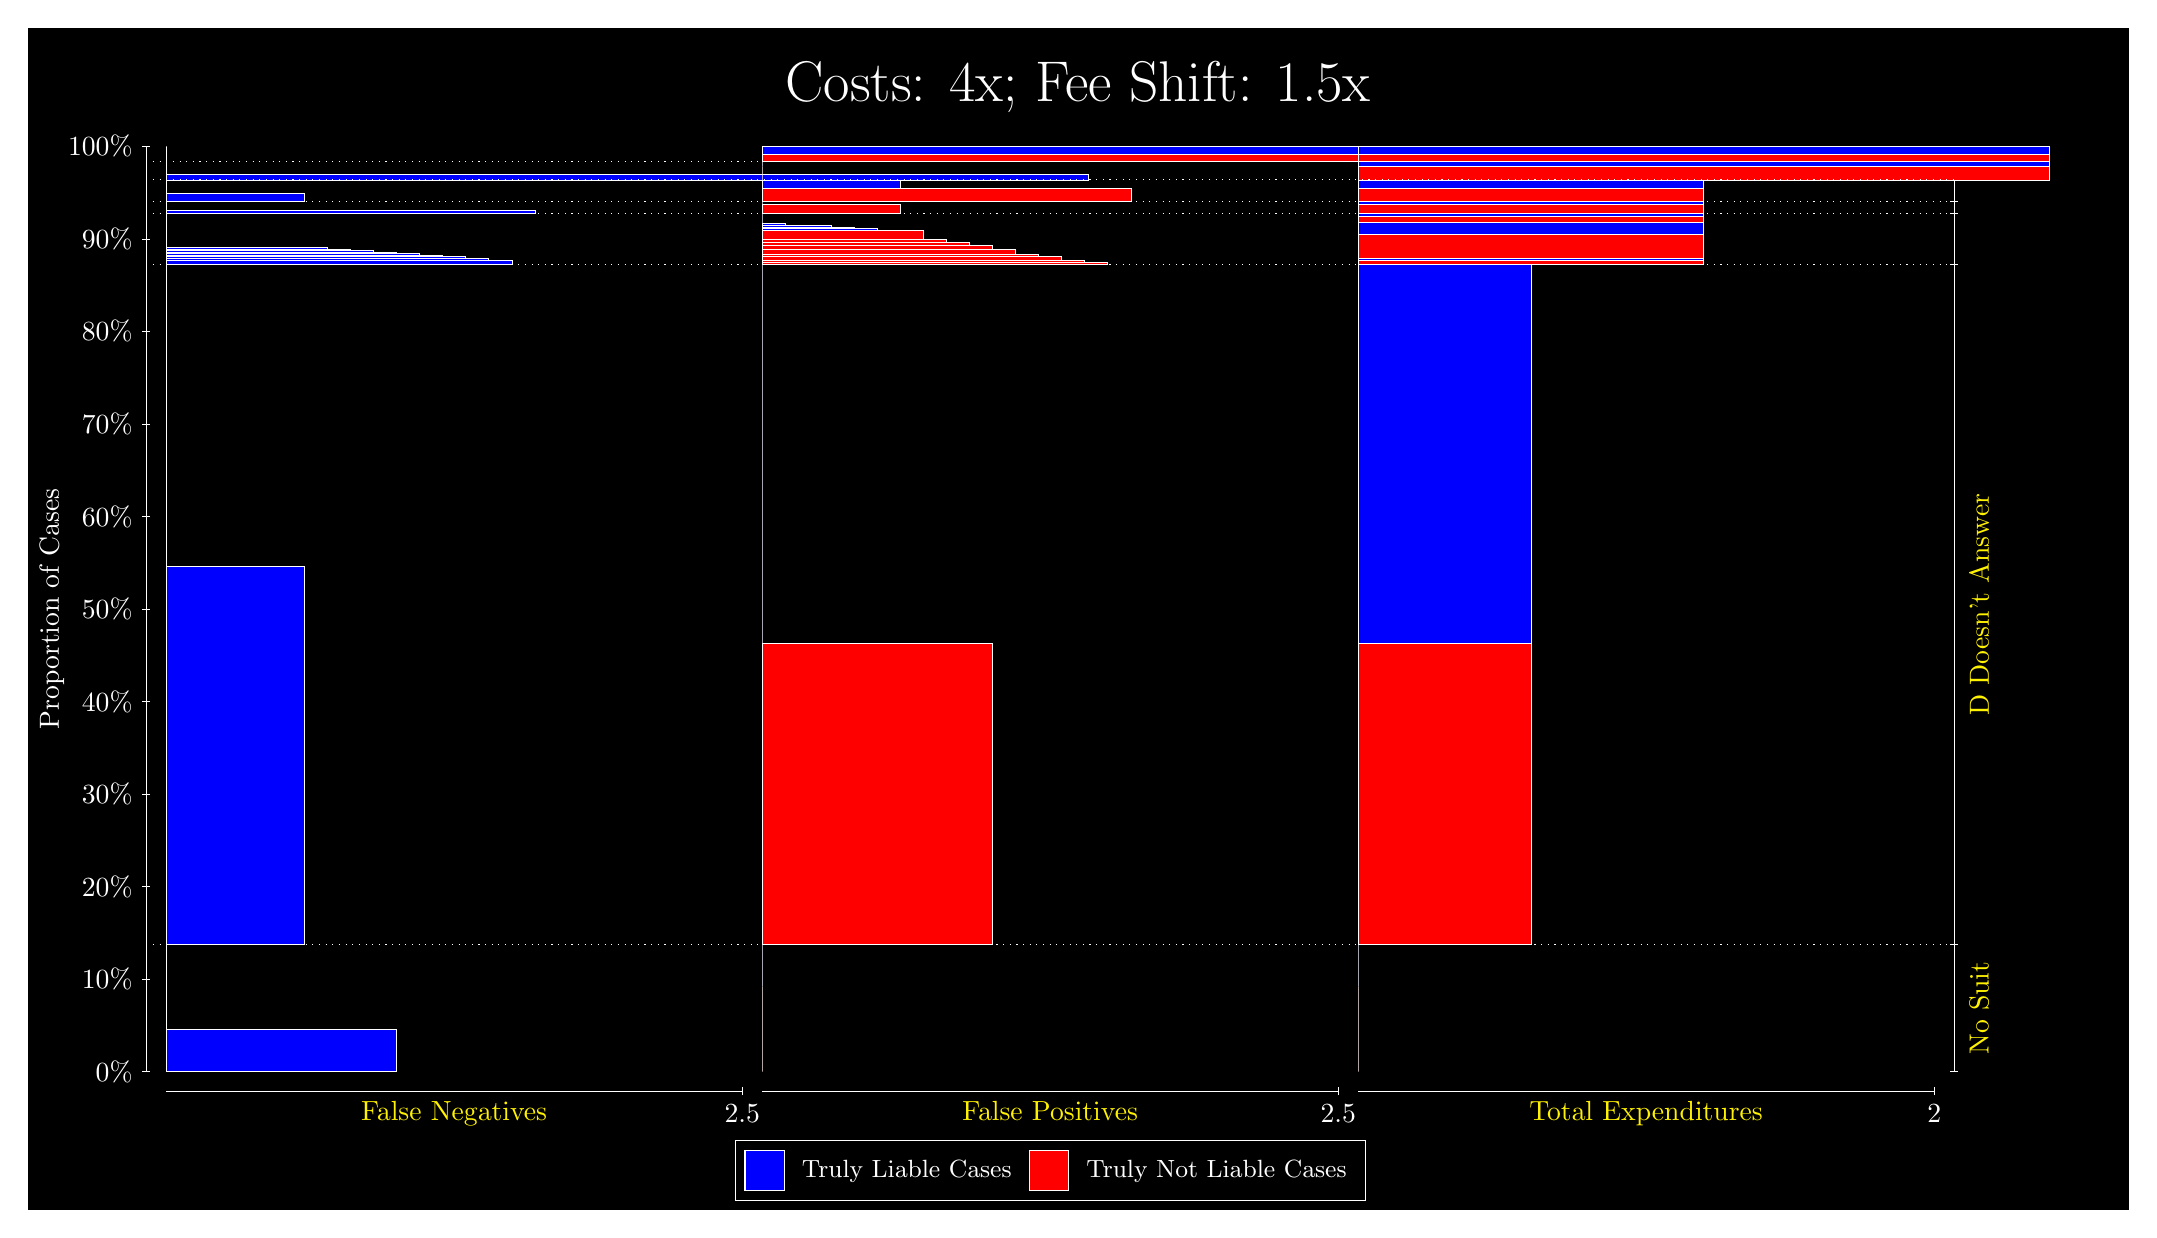
\begin{tikzpicture}
\draw[fill=black] (0,0) rectangle (26.667,15);
\draw[text=white] (0,13.5) rectangle (26.667,15) node[midway] {\huge Costs: 4x; Fee Shift: 1.5x};
\draw[white, very thin] (1.5,1.75) -- (1.5,13.5);
\node[rotate=90, text=white, anchor=center] at (0.3, 7.625) {Proportion of Cases};
\draw[white, very thin] (1.45,1.75) -- (1.55,1.75);
\node[text=white, anchor=east] at (1.45, 1.75) {0\%};
\draw[white, very thin] (1.45,2.925) -- (1.55,2.925);
\node[text=white, anchor=east] at (1.45, 2.925) {10\%};
\draw[white, very thin] (1.45,4.1) -- (1.55,4.1);
\node[text=white, anchor=east] at (1.45, 4.1) {20\%};
\draw[white, very thin] (1.45,5.275) -- (1.55,5.275);
\node[text=white, anchor=east] at (1.45, 5.275) {30\%};
\draw[white, very thin] (1.45,6.45) -- (1.55,6.45);
\node[text=white, anchor=east] at (1.45, 6.45) {40\%};
\draw[white, very thin] (1.45,7.625) -- (1.55,7.625);
\node[text=white, anchor=east] at (1.45, 7.625) {50\%};
\draw[white, very thin] (1.45,8.8) -- (1.55,8.8);
\node[text=white, anchor=east] at (1.45, 8.8) {60\%};
\draw[white, very thin] (1.45,9.975) -- (1.55,9.975);
\node[text=white, anchor=east] at (1.45, 9.975) {70\%};
\draw[white, very thin] (1.45,11.15) -- (1.55,11.15);
\node[text=white, anchor=east] at (1.45, 11.15) {80\%};
\draw[white, very thin] (1.45,12.325) -- (1.55,12.325);
\node[text=white, anchor=east] at (1.45, 12.325) {90\%};
\draw[white, very thin] (1.45,13.5) -- (1.55,13.5);
\node[text=white, anchor=east] at (1.45, 13.5) {100\%};

\draw[white, very thin] (24.457,1.75) -- (24.457,13.5);
\draw[white, very thin] (24.407,1.75) -- (24.507,1.75);
\node[anchor=west] at (24.407, 1.75) {};
\draw[white, very thin] (24.407,3.3602) -- (24.507,3.3602);
\node[anchor=west] at (24.407, 3.3602) {};
\draw[white, very thin] (24.407,11.996) -- (24.507,11.996);
\node[anchor=west] at (24.407, 11.996) {};
\draw[white, very thin] (24.407,12.65) -- (24.507,12.65);
\node[anchor=west] at (24.407, 12.65) {};
\draw[white, very thin] (24.407,12.797) -- (24.507,12.797);
\node[anchor=west] at (24.407, 12.797) {};
\draw[white, very thin] (24.407,13.073) -- (24.507,13.073);
\node[anchor=west] at (24.407, 13.073) {};
\draw[white, very thin] (24.407,13.311) -- (24.507,13.311);
\node[anchor=west] at (24.407, 13.311) {};
\draw[white, very thin] (24.407,13.5) -- (24.507,13.5);
\node[anchor=west] at (24.407, 13.5) {};

\draw[white, very thin, fill=blue] (1.75,1.75) rectangle (4.6775,2.2834);
\draw[white, very thin, fill=red] (1.75,2.2834) rectangle (1.75,3.3602);
\draw[white, very thin, fill=blue] (1.75,3.3602) rectangle (3.5065,8.1695);
\draw[white, very thin, fill=red] (1.75,8.1695) rectangle (1.75,11.996);
\draw[white, very thin, fill=blue] (1.75,11.996) rectangle (6.1413,12.059);
\draw[white, very thin, fill=blue] (1.75,12.059) rectangle (5.8486,12.076);
\draw[white, very thin, fill=blue] (1.75,12.076) rectangle (5.5558,12.098);
\draw[white, very thin, fill=blue] (1.75,12.098) rectangle (5.2631,12.119);
\draw[white, very thin, fill=blue] (1.75,12.119) rectangle (4.9703,12.145);
\draw[white, very thin, fill=blue] (1.75,12.145) rectangle (4.6775,12.155);
\draw[white, very thin, fill=blue] (1.75,12.155) rectangle (4.3848,12.177);
\draw[white, very thin, fill=blue] (1.75,12.177) rectangle (4.092,12.194);
\draw[white, very thin, fill=blue] (1.75,12.194) rectangle (3.7993,12.215);
\draw[white, very thin, fill=red] (1.75,12.215) rectangle (1.75,12.65);
\draw[white, very thin, fill=blue] (1.75,12.65) rectangle (6.4341,12.69);
\draw[white, very thin, fill=red] (1.75,12.69) rectangle (1.75,12.797);
\draw[white, very thin, fill=blue] (1.75,12.797) rectangle (3.5065,12.907);
\draw[white, very thin, fill=red] (1.75,12.907) rectangle (1.75,13.073);
\draw[white, very thin, fill=blue] (1.75,13.073) rectangle (13.46,13.139);
\draw[white, very thin, fill=red] (1.75,13.139) rectangle (1.75,13.311);
\draw[white, very thin, fill=red] (1.75,13.311) rectangle (1.75,13.401);
\draw[white, very thin, fill=blue] (1.75,13.401) rectangle (1.75,13.5);
\draw[white, very thin, fill=red] (9.3189,1.75) rectangle (9.3189,2.8268);
\draw[white, very thin, fill=blue] (9.3189,2.8268) rectangle (9.3189,3.3602);
\draw[white, very thin, fill=red] (9.3189,3.3602) rectangle (12.246,7.1867);
\draw[white, very thin, fill=blue] (9.3189,7.1867) rectangle (9.3189,11.996);
\draw[white, very thin, fill=red] (9.3189,11.996) rectangle (13.71,12.024);
\draw[white, very thin, fill=red] (9.3189,12.024) rectangle (13.417,12.056);
\draw[white, very thin, fill=red] (9.3189,12.056) rectangle (13.125,12.104);
\draw[white, very thin, fill=red] (9.3189,12.104) rectangle (12.832,12.135);
\draw[white, very thin, fill=red] (9.3189,12.135) rectangle (12.539,12.195);
\draw[white, very thin, fill=red] (9.3189,12.195) rectangle (12.246,12.24);
\draw[white, very thin, fill=red] (9.3189,12.24) rectangle (11.954,12.287);
\draw[white, very thin, fill=red] (9.3189,12.287) rectangle (11.661,12.318);
\draw[white, very thin, fill=red] (9.3189,12.318) rectangle (11.368,12.431);
\draw[white, very thin, fill=blue] (9.3189,12.431) rectangle (10.783,12.453);
\draw[white, very thin, fill=blue] (9.3189,12.453) rectangle (10.49,12.47);
\draw[white, very thin, fill=blue] (9.3189,12.47) rectangle (10.197,12.492);
\draw[white, very thin, fill=blue] (9.3189,12.492) rectangle (9.9044,12.502);
\draw[white, very thin, fill=blue] (9.3189,12.502) rectangle (9.6116,12.527);
\draw[white, very thin, fill=blue] (9.3189,12.527) rectangle (9.3189,12.65);
\draw[white, very thin, fill=red] (9.3189,12.65) rectangle (11.075,12.758);
\draw[white, very thin, fill=blue] (9.3189,12.758) rectangle (9.3189,12.797);
\draw[white, very thin, fill=red] (9.3189,12.797) rectangle (14.003,12.964);
\draw[white, very thin, fill=blue] (9.3189,12.964) rectangle (11.075,13.073);
\draw[white, very thin, fill=red] (9.3189,13.073) rectangle (9.3189,13.246);
\draw[white, very thin, fill=blue] (9.3189,13.246) rectangle (9.3189,13.311);
\draw[white, very thin, fill=red] (9.3189,13.311) rectangle (21.029,13.401);
\draw[white, very thin, fill=blue] (9.3189,13.401) rectangle (18.102,13.5);
\draw[white, very thin, fill=red] (16.888,1.75) rectangle (16.888,2.8268);
\draw[white, very thin, fill=blue] (16.888,2.8268) rectangle (16.888,3.3602);
\draw[white, very thin, fill=red] (16.888,3.3602) rectangle (19.083,7.1867);
\draw[white, very thin, fill=blue] (16.888,7.1867) rectangle (19.083,11.996);
\draw[white, very thin, fill=red] (16.888,11.996) rectangle (21.279,12.056);
\draw[white, very thin, fill=blue] (16.888,12.056) rectangle (21.279,12.081);
\draw[white, very thin, fill=red] (16.888,12.081) rectangle (21.279,12.377);
\draw[white, very thin, fill=blue] (16.888,12.377) rectangle (21.279,12.532);
\draw[white, very thin, fill=red] (16.888,12.532) rectangle (21.279,12.612);
\draw[white, very thin, fill=blue] (16.888,12.612) rectangle (21.279,12.65);
\draw[white, very thin, fill=red] (16.888,12.65) rectangle (21.279,12.758);
\draw[white, very thin, fill=blue] (16.888,12.758) rectangle (21.279,12.797);
\draw[white, very thin, fill=red] (16.888,12.797) rectangle (21.279,12.964);
\draw[white, very thin, fill=blue] (16.888,12.964) rectangle (21.279,13.073);
\draw[white, very thin, fill=red] (16.888,13.073) rectangle (25.67,13.246);
\draw[white, very thin, fill=blue] (16.888,13.246) rectangle (25.67,13.311);
\draw[white, very thin, fill=red] (16.888,13.311) rectangle (25.67,13.401);
\draw[white, very thin, fill=blue] (16.888,13.401) rectangle (25.67,13.5);
\draw[white, dotted] (1.5,3.3602) -- (24.457,3.3602);
\draw[white, dotted] (1.5,11.996) -- (24.457,11.996);
\draw[white, dotted] (1.5,12.65) -- (24.457,12.65);
\draw[white, dotted] (1.5,12.797) -- (24.457,12.797);
\draw[white, dotted] (1.5,13.073) -- (24.457,13.073);
\draw[white, dotted] (1.5,13.311) -- (24.457,13.311);
\draw[white, very thin] (1.75,1.5) -- (9.0689,1.5);
\node[text=yellow, anchor=north] at (5.4094, 1.5) {False Negatives};
\draw[white, very thin] (9.0689,1.45) -- (9.0689,1.55);
\node[text=white, anchor=north] at (9.0689, 1.45) {2.5};

\draw[white, very thin] (9.3189,1.5) -- (16.638,1.5);
\node[text=yellow, anchor=north] at (12.978, 1.5) {False Positives};
\draw[white, very thin] (16.638,1.45) -- (16.638,1.55);
\node[text=white, anchor=north] at (16.638, 1.45) {2.5};

\draw[white, very thin] (16.888,1.5) -- (24.207,1.5);
\node[text=yellow, anchor=north] at (20.547, 1.5) {Total Expenditures};
\draw[white, very thin] (24.207,1.45) -- (24.207,1.55);
\node[text=white, anchor=north] at (24.207, 1.45) {2};

\node[text=yellow, centered, rotate=90] at (24.777, 2.5551) {No Suit};
\node[text=yellow, centered, rotate=90] at (24.777, 7.6781) {D Doesn't Answer};






\draw (12.978300999999998,1.5) node[draw=none] (baseCoordinate) {};
\begin{scope}[align=center]
        \matrix[scale=0.5, draw=white, below=0.5cm of baseCoordinate, nodes={draw}, column sep=0.1cm]{
            \node[rectangle, draw, minimum width=0.5cm, minimum height=0.5cm, fill=blue] {}; &
            \node[draw=none, font=\small, text=white] (B) {Truly Liable Cases}; &
            \node[rectangle, draw, minimum width=0.5cm, minimum height=0.5cm, fill=red] {}; &
            \node[draw=none, font=\small, text=white] (B) {Truly Not Liable Cases}; \\
            };
\end{scope}

\end{tikzpicture}
\end{document}